\documentclass[10pt,twocolumn,letterpaper]{article}

\usepackage{cvpr}
\usepackage{times}
\usepackage{epsfig}
\usepackage{graphicx}
\usepackage{amsmath}
\usepackage{amssymb}

% Include other packages here, before hyperref.

% If you comment hyperref and then uncomment it, you should delete
% egpaper.aux before re-running latex.  (Or just hit 'q' on the first latex
% run, let it finish, and you should be clear).
\usepackage[breaklinks=true,bookmarks=false]{hyperref}

\cvprfinalcopy % *** Uncomment this line for the final submission

%\def\cvprPaperID{****} % *** Enter the CVPR Paper ID here
%\def\httilde{\mbox{\tt\raisebox{-.5ex}{\symbol{126}}}}

% Pages are numbered in submission mode, and unnumbered in camera-ready
%\ifcvprfinal\pagestyle{empty}\fi
\setcounter{page}{1}
\begin{document}

\title{Adapting Rainbow DQN to Atari games}

\author{Willi Menapace\\
Ms-Pacman\\
{\tt\small willi.menapace@studenti.unitn.it}
% For a paper whose authors are all at the same institution,
% omit the following lines up until the closing ``}''.
% Additional authors and addresses can be added with ``\and'',
% just like the second author.
% To save space, use either the email address or home page, not both
\and
Luca Zanella\\
Atlantis\\
{\tt\small luca.zanella-3@studenti.unitn.it}
\and
Daniele Giuliani\\
Demon Attack\\
{\tt\small daniele.giuliani@studenti.unitn.it}
}

\maketitle
%\thispagestyle{empty}

%%%%%%%%% ABSTRACT


%%%%%%%%% BODY TEXT
\section{Introduction}

Reinforcement Learning is one of the most active research area in the deep learning community. Its main challenge is finding a way to optimize a target function, usually the cumulative sum of rewards obtained through the policy, through experience and without explicit supervision. This technology finds a variety of possible applications that include continuous control systems such as autonomous cars or robotic arms, stock trading agents or videogame agents. However, despite its relevancy, it is only recently that major improvements have come from the research community allowing the achievement of significant results.
In particular, the attention of our group was caught by the victory of novel RL systems in exceptionally challenging games such as Starcraft 2 (DeepMind, December 2018) and Dota 2 (OpenAI, April 2019) against professional players. In order to take a glimpse into the the world of reinforcement learning and try to give a little contribution to the field, we revisit the DQN architecture introduced by DeepMind in \cite{DBLP:journals/corr/MnihKSGAWR13}, and improved upon in \cite{DBLP:journals/corr/abs-1710-02298}. The objective is to train and tune agents able to play at human skill level or better a set of chosen Atari games using only raw pixel input, namely Ms-Pacman, Atlantis and Demon Attack. The task is expected to be particularly challenging for the Ms-Pacman game as shown in \cite{humancontrol} where the plain DQN approach is able to achieve only a reported 13\% performance compared to a human player and proficient systems in this game usually take as input the internal game state rather than pixel output.
Another challenging element is computing time. RL training phases are computationally expensive and reference results taken from \cite{DBLP:journals/corr/abs-1710-02298} are given after 200 million training iterations. From our benchmarks and codebase, a system equipped with a RTX 2070 GPU can process ~70 frames per second, giving a projected time of 33 GPU days for training in order to emulate the results. This is a prohibitive time amount, so we need to take steps to increase convergence speed on each particular game.

%-------------------------------------------------------------------------

\subsection{Proposed Method}

We start with a tensorflow based hand implementation of a DQN as described in \cite{DBLP:journals/corr/MnihKSGAWR13} and test it on Ms-Pacman. We take care of implementing many of the engineering tricks explained in the paper such as reward clipping, frameskipping, frame stacking, different gray conversions and image rescalings. We also experiment with using a Huber loss function instead of MSE to avoid too aggressive weights updates. Special care has also been taken to optimize the memory footprint of the replay buffer by storing each preprocessed frame only once and in int8 format. This allow us to use a large 1M frames replay buffer that can fit in less than 10GB of memory.

As shown in \cite{humancontrol}, Ms-Pacman is a challenging environment for reinforcement learning algorithms due to its complexity. It requires the agent to be able to navigate in a maze to chase remaining dots to eat while avoiding being eaten by ghosts. An added complexity is given by the fact that after eating a special `pill' the ghosts become eatable for a limited amount of time and the agent needs to identify these timeframes and proactively chase ghosts in order to take them out.

We run the trained agent for 50 episodes, measuring the average game score and, unsurprisingly, this simple architecture is not satisfying, so we decide to implement the optimizations proposed in \cite{DBLP:journals/corr/abs-1710-02298} and generally referred to as Rainbow DQN. Due to the complexity of the first implementation and the desire to migrate our codebase to the pytorch environment, we decide to base our implementation on top of the ptan agent library \cite{ptan}, taking \cite{packtrepo} as the initial codebase.

We start by implementing and integrating together the N-Step, Double DQN and Noisy Layers optimizations, noticing improvements in average reward of the trained agent. In particular the $\epsilon$-greedy exploration strategy proposed in \cite{DBLP:journals/corr/MnihKSGAWR13} and replaced by the noisy layers in this implementation is particularly unsuited for Ms-Pacman. This exploration strategy causes a random action to happen with probability $1 - \epsilon$ and is necessary to avoid the agent from blocking in loops of actions while playing, but also causes death every time the agent is chased by a ghost, with the agent escaping successfully until the moment when a random action causes the agent to run into the ghost and be eaten.
Noisy layers, on the other hand, work by perturbing the estimation of qvalues. When the agent is stuck in a loop of actions determined by similar qvalues, the agent is still able to escape it thanks to the perturbations introduced by noisy layers, but when it is chased by a ghost and qvalues are far away from each other, the qvalue perturbations introduced by noise do not affect the choice of the agent to escape from the ghost.

Encouraged by the results, we decide to continue integrating the remaining rainbow improvements into our DQN architecture, namely the Prioritized Replay Buffer, Distributional DQN and Dueling DQN, but the likelihood to introduce subtle bugs in our implementation due to the complexity of the task lead us to use the rainbow agent implementation provided by our library as a base for the rest of the experiments.

At this point each group member proceeds to tune the model to its environment.

\subsubsection{Ms-Pacman}
We start by performing a hyperparameter search on the model in order to tune the original hyperparameters proposed in \cite{DBLP:journals/corr/abs-1710-02298}. The search is complicated by the very long training times needed to see the effects of each modification. In particular we notice instability when training the model with the proposed learning rate of $6.25e-5$, so we lower it to $2e-5$ obtaining more consistent gains in reward over time. We also set the prioritized buffer $\beta$ annealing curve to end at 3M frames in order to enable the model to have a large initial time where the prioritized buffer can be more effective. Moreover the target network is updated every 10k frames like in the initial plain DQN implementation instead of the proposed 32k to stimulate faster convergence. The buffer size is set to 1M frames when training on local machines, while it is slightly reduced when training on Google Colab due to memory limitations.

The agent trained on the rainbow model still shows unsatisfying behaviors after 38 hours of training. Training dynamics are shown in Fig. \ref{fig:rewardPacmanPlainRainbow}. The agent learns to successfully eat dots across the maze and to eat the special pills that allow it to eat ghosts, but when the special pills terminate and few dots remain in the maze the agent seems unable to detect the presence of attacking ghosts and runs into them.
An analysis of qvalues output by the network show the reason for the behavior. The reward system used for training clips rewards in the range (-1, 1), but never assigns a negative reward to the agent upon death. In an environment such as OpenAI Cartpole, where the agent continuously receives rewards, this is not a problem because death prevents the agent to accumulate future rewards, so qvalues diminish for actions that will lead to death. In our situation however, when there are no dots and special pills in close proximity, the correct qvalue to estimate is 0 for every action. When a ghost approaches, the correct qvalue to estimate is still 0 for every action due to the absence of death penalties, so the agent may well decide to run into the ghost. Moreover, in the original game, there is a difference in color from ghosts that are eatable and ghosts that are not, but due to grayscale conversion we notice that there is only a subtle difference between eatable and not eatable ghosts which may further damage training.

\begin{figure}
	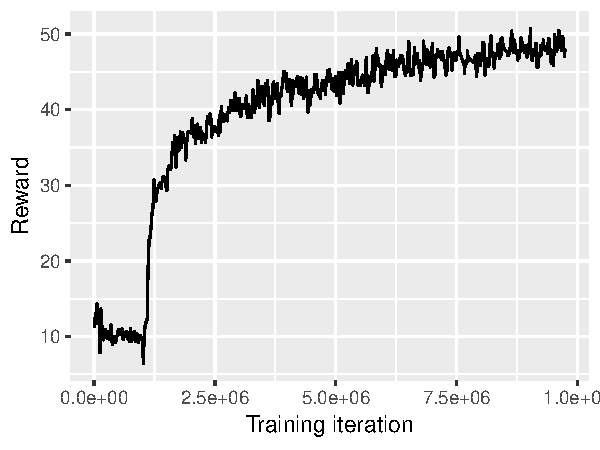
\includegraphics[width=\linewidth]{run_results/plain_rainbow_reward.pdf}
	\caption{Training reward dynamics of the pacman agent after the first reshaping. The reward refers to the average clipped reward obtained by the agent in the last 100 episodes. The reward increases slowly, but the agent is unaware of ghosts when the number of dots reduces, leading it to unfrequently complete the first level.}
	\label{fig:rewardPacmanPlainRainbow}
\end{figure}

In order to address this problems we preprocess each frame in order to make eatable ghosts of a distinguishable gray tonality and we use a common technique in RL called reward reshaping, which consists in changing the rewards in order to drive the policy towards the wanted direction.
Care has been taken in order not for expected qvalues to saturate the boundaries imposed to qvalues by the Distributional DQN modification. For the subsequent attempt the reward policy was reshaped in this way:
\begin{itemize}
	\item Eating dot $1 \rightarrow 0.5$
	\item Eating pill $1 \rightarrow 1$
	\item Eating ghost $1 \rightarrow 2$
	\item Eating fruit $1 \rightarrow 0.5$
	\item Being eaten $0 \rightarrow -7$
	\item Finishing level $1 \rightarrow 7$
\end{itemize}

\begin{figure}
	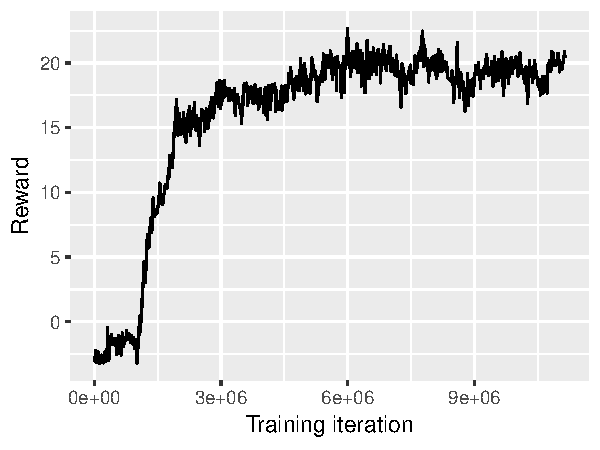
\includegraphics[width=\linewidth]{run_results/reward_afraid.pdf}
	\caption{Training reward dynamics of the pacman agent after the first reshaping. The reward refers to the average reshaped reward obtained by the agent in the last 100 episodes. The reward does not increase further after 6M frames because the agent is hindered in chasing the last dots to eat due to high death penalization and does not get to the second level.}
	\label{fig:rewardPacmanAfraid}
\end{figure}

The results obtained with these settings, however, were not satisfying. The training dynamics are shown in Fig. \ref{fig:rewardPacmanAfraid}. An analysis of the behavior of the agent in fact highlighted that, due to the high death penalization, the agent was so hindered to get close to a ghost that it always tried to hide away from them, ignoring nearby dots to eat and not making progress. Moreover, due to the relatively high special pill and ghost eating rewards, the agent tended to immediately eat all the available special pills, and be very aggressive with regards to eatable ghosts. While this strategy provided high game scores, our main objective was to make progress through different levels, so rewards were reshaped again to encourage a more gentle behavior:
\begin{itemize}
	\item Eating dot $0.5 \rightarrow 0.5$
	\item Eating pill $1 \rightarrow 0$
	\item Eating ghost $2 \rightarrow 1.5$
	\item Eating fruit $0.5 \rightarrow 0.5$
	\item Being eaten $-7 \rightarrow -2$
	\item Finishing level $7 \rightarrow 4$
\end{itemize}

Notably, we didn't reward the agent for eating special pills in order not to encourage it to eat them in close succession, reduced the reward for eating ghosts and considerably reduced the penalty for being eaten.

This settings proved successful. After 90 hours of training the agent proactively searches dots to eat in the maze, eats special pills at reasonable timeframes, hunts eatable ghosts and run away from dangerous ones.
In order to aid convergence we also reduce the learning rate from $2e-5$ to $5e-6$ after 44 training hours and 11.3M training iterations and from $5e-6$ to $1.25e-6$ after 16.5M training iterations and 74 hours of training. Training reward dynamics are shown in Fig. \ref{fig:rewardPacmanFinal}.

\begin{figure}
	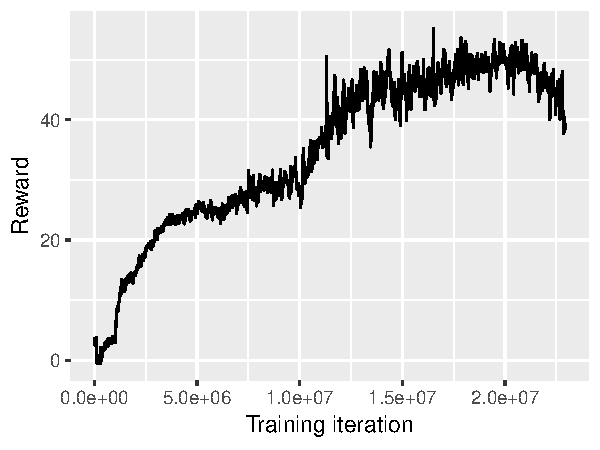
\includegraphics[width=\linewidth]{run_results/final_reward.pdf}
	\caption{Training reward dynamics of last pacman agent. The reward refers to the average reshaped reward obtained by the agent in the last 100 episodes. The reward increases fastly in the first million of iterations and then stabilizes. When at 10M iterations the agent learns how to clear all the dots and pass to the second level the reward begins to grow quickly again.}
	\label{fig:rewardPacmanFinal}
\end{figure}

\subsubsection{Atlantis}
\label{atlantis}
The choice of Atlantis is based on the $449.9\%$ performance obtained by the plain DQN approach compared to a human player as shown in \cite{humancontrol}.
 
The game consists in defending the city of Atlantis, made of three defense posts that can be used by the player to attack enemies and six Atlantean installations, from the Gorgon vessels. The game ends when the Acropolis Command Post and all six of Atlantis' installations are destroyed. 

In the original Rainbow DQN, observations are grey-scaled and cropped to $84$ x $84$ pixels \cite{DBLP:journals/corr/abs-1710-02298}, however, this setting on Atlantis eliminates a relevant portion of the sky and maintains irrelevant information at the bottom such as the score. Based on that, we decided to crop observations to $92$ x $84$ pixels maintaining only signicant information in the frame.

Gorgon vessels circle down from the highest level to the one closest to Atlantis and can only fire their deathray when close to the city. Since the first hours of training, the agent learns to successfully destroy Gorgon vessels, reaching scores above the ones obtained by a professional human games tester as shown in \cite{humancontrol}.  One of the most notable aspects encountered during the training was the discovery of a bug in the system that prevents one of the six Atlantean installations to be demolished. Although this strategy leads to the highest possible game score, the main objective was to make the agent strong enough to not rely on this shortcut and we decided to proceed with the training. This choice proved to be successful in improving the policy of the agent: the game score obtained is still the highest possible, but now the agent does not rely on the bug and concludes the game episode with all seven installations being untoched for most of the time. Another significant aspect is that the agent mainly uses the Acropolis Command Post and the right sentry post to defend all the Atlantis' installations.

\subsubsection{Demon Attack}
\label{demon_attack}
The third game to which we try to apply the Rainbow DQN architecture is Demon Attack. The game mechanics are pretty simple. The player controls a space ship which can be moved horizontally across the playing field. The objective is to shoot down all the enemy spaceships, while avoiding their attacks. As the game progresses the enemies become stronger and stronger, they gain movement speed and use different attack patterns.

Initially, the training of the network for this game was done using Google Colab due to the fact that some of our laptops were not powerful enough to sustain the training at an acceptable speed. Unfortunately, Google Colab has strict limits on how long a program can run. This meant that we had to restart the training every few hours slowing down the process. Furthermore, we noticed that checkpoint restarts cause problems with the implementation of the prioritized replay buffer used by our library, probably due to a sub-optimal initialization of buffer weights. Although it would be possible to save the state of the buffer as a part of the checkpoint, we decided to resort to the plain replay buffer to avoid saving a component of the size of tens of gigabytes.

As a second approach, we retrained the whole network during the weekend using a more powerful local machine. This time, we trained the network for approximately 72 hours consecutively on a machine with a GTX 960 GPU which, although not as performing as the RTX 2070 and far from the performance of the Tesla T4 provided by Colab, was still able to process 20 frames per second. With this approach, we could also make use of the prioritized buffer which, as described in the result section, improved noticeably the performance of the network.

\subsection{Results}

\subsubsection{Ms-Pacman}

Table \ref{tab:pacman_results} shows average scores obtained by each agent we trained on Ms-Pacman.

\begin{table}
	\begin{center}
		\begin{tabular}{ |c|c|c|c| } 
			\hline
			 & Plain DQN & Rainbow DQN & Our \\ 
			 \hline
			Mean score & 1880 & 2267 & 5145 \\
			Std dev. & 448 & 504 & 866 \\
			Samples & 50 & 50 & 50 \\
			Train frames & 11.4M & 9.7M & 22.9M \\
			Train time & ~45h & ~38h & ~90h \\
			\hline
		\end{tabular}
	\end{center}
	\caption{Ms-Pacman agent results. Results refer to the point in time when the agent stopped showing improvements in gathered reward.}
	\label{tab:pacman_results}
\end{table}

Notably, the reward reshaping and frame preprocessing approach we used to train our final agent version allowed the network to obtain an average score of 5145 after 22.9M training iteration. For comparison \cite{DBLP:journals/corr/abs-1710-02298} reports an average 5380.4 score on Ms-Pacman after 200M training iterations which we consider a success given our limited computational resources.
The score corresponds to reaching on average the end of level 2 and sometimes reaching level 3. Interestingly, Ms-Pacman level 3 has a different color pattern and maze structure which may be the reason why the agent struggles to gather further reward. Modifying the Ms-Pacman emulator to start from level 3 instead of level 1 with a certain probability may allow the agent to gather more samples from this level and continue its improvements.
Moreover, \cite{DBLP:journals/corr/WangFL15} and \cite{humancontrol} reports an average human score for Ms-Pacman of respectively 6951.6 and 15693, meaning we are still not able to reach human level behavior, but the result is satisfying.

\subsubsection{Atlantis}
Table \ref{tab:atlantis_results} shows average scores obtained by the agent we trained on Atlantis. 

\begin{table}
	\begin{center}
		\begin{tabular}{ |c|c|c|c| } 
			\hline
			& Our Rainbow \\ 
			\hline
			Mean score & 2,609,433.3 \\
			Std dev. & 1,250,245.2 \\
			Samples & 42 \\
			Train frames & 6.6M \\
			Train time & ~25h \\
			\hline
		\end{tabular}
	\end{center}
	\caption{Atlantis agent results.}
	\label{tab:atlantis_results}
\end{table}

DeepMind reports an average score for Rainbow on Atlantis over 200 testing episodes of $826,659.5$ \cite{DBLP:journals/corr/abs-1710-02298}. The frame preprocessing approach we used to train our agent allowed the network to obtain an average score of $2,609,433.3$ after $6.6$M training iterations without exploiting the bug mentioned in \ref{atlantis} despite the left sentry post is not as precise as the others.  Proceeding with the training of the network should solve this problem.

\subsubsection{Demon Attack}

\begin{table}
	\begin{center}
		\begin{tabular}{ |c|c|c|c| } 
			\hline
			& Rainbow & Rainbow + Prio \\ 
			\hline
			Mean score & 6828 & 10291\\
			Std dev. & 1812 & 4165\\
			Samples & 100 & 100\\
			Train frames & 6.9M & 4.1M\\
			Train time & 29h (on Tesla T4) & 72h (on GTX 960)\\
			\hline
		\end{tabular}
	\end{center}
	\caption{Demon Attack agents results.}
	\label{tab:da_result}
\end{table}
All of the results are summarized in the Table \ref{tab:da_result}.

With the first approach we were able to obtain a decent score after approximately $29$ hours of training on Google Colab. At this point, the network performance was not improving consistently even with more training time. Our intuition was that the network had difficulty defeating the stronger enemies encountered later in the game, due to the fact that their attack pattern was different from all the one seen up to that point and the network did not encounter this enemy frequently enough to be able to devise a good strategy for defeating them.

With the second approach instead after $72$ hours of training (and only $4.1$M frames processed given the outdated hardware) we were able to improve the mean score by a considerable amount over the previous attempt, this is a great result if we take into account the fact that fewer frames were processed by the network.

The scores obtained are lower than the one obtained by \cite{DBLP:journals/corr/abs-1710-02298}. In fact, we noticed that the network had a problem learning one particular attack pattern used in the late game which is visually similar to the previous attack but works differently: while all other attacks move only vertically, this attack can track the player and follow him horizontally, so for the agent it is more difficult to avoid.

Because of the huge time requirement and hardware availability, we were not able to train the network any further. Nevertheless, the results obtained are encouraging and training even more the network would probably allow the agent to learn the advanced attack patterns and obtain much higher scores.

{\small
\bibliographystyle{ieee}
\bibliography{egbib}
}

\end{document}
